\documentclass[aspectratio=169,12pt,t]{beamer}

% --- Theme: Metropolis (modern, clean) ---
\usetheme[progressbar=frametitle,numbering=fraction,block=fill]{metropolis}

% --- Fira Sans font (install texlive-fonts-extra if missing) ---
\IfFileExists{FiraSans.sty}{\usepackage[sfdefault]{FiraSans}}{}

% --- Light background with warm accent ---
\definecolor{mDarkTeal}{RGB}{35,55,59}
\definecolor{mLightBrown}{RGB}{235,228,216}
\definecolor{mAccent}{RGB}{140,70,20}

\setbeamercolor{normal text}{fg=mDarkTeal,bg=white}
\setbeamercolor{alerted text}{fg=mAccent}
\setbeamercolor{frametitle}{bg=mDarkTeal,fg=white}
\setbeamercolor{progress bar}{fg=mAccent,bg=mLightBrown}
\setbeamercolor{title separator}{fg=mAccent}
\setbeamercolor{progress bar in head/foot}{fg=mAccent,bg=mLightBrown}
\setbeamercolor{progress bar in section page}{fg=mAccent,bg=mLightBrown}

% --- Packages ---
\usepackage[utf8]{inputenc}
\usepackage{amsmath,amssymb,amsthm}
\usepackage{mathrsfs}
\usepackage{tikz}
\usetikzlibrary{arrows.meta,positioning,calc,decorations.pathreplacing,shapes,patterns}
\usepackage{pgfplots}
\pgfplotsset{compat=1.18}

% --- Semi-transparent white highlight for text on top of background images ---
\usepackage[most]{tcolorbox}

% Inline highlight: \hl{short text}
\newtcbox{\hl}{%
  nobeforeafter, tcbox raise base,
  colback=white, opacityback=0.6,
  colframe=white, opacityframe=0,
  sharp corners, boxsep=2pt, left=3pt, right=3pt, top=2pt, bottom=2pt%
}

% Block highlight: \begin{hlbox} ... \end{hlbox}  (multi-line, paragraphs, itemize)
\newtcolorbox{hlbox}[1][]{%
  enhanced, breakable,
  colback=white, opacityback=0.6,
  colframe=white, opacityframe=0,
  boxsep=3pt, left=6pt, right=6pt, top=4pt, bottom=4pt,
  sharp corners,
  {#1}%
}

% --- Custom colors for content types ---
\definecolor{defcolor}{RGB}{25,85,120}
\definecolor{thmcolor}{RGB}{140,35,35}
\definecolor{proofcolor}{RGB}{35,100,50}
\definecolor{excolor}{RGB}{140,75,10}
\definecolor{remcolor}{RGB}{90,90,90}

% --- Beamer blocks for mathematical content types (semi-transparent) ---
\tcbset{hlblockbase/.style={
  enhanced, breakable,
  coltitle=white, fonttitle=\bfseries,
  opacitybacktitle=0.8, opacityback=0.6,
  opacityframe=0,
  sharp corners,
  boxsep=1pt, left=5pt, right=5pt, top=2pt, bottom=2pt,
  toptitle=1pt, bottomtitle=1pt
}}

\newtcolorbox{defblock}[1]{hlblockbase, title={#1},
  colbacktitle=defcolor, colback=defcolor!15, colframe=defcolor}
\newtcolorbox{thmblock}[1]{hlblockbase, title={#1},
  colbacktitle=thmcolor, colback=thmcolor!15, colframe=thmcolor}
\newtcolorbox{proofblock}[1]{hlblockbase, title={#1},
  colbacktitle=proofcolor, colback=proofcolor!15, colframe=proofcolor}
\newtcolorbox{exblock}[1]{hlblockbase, title={#1},
  colbacktitle=excolor, colback=excolor!15, colframe=excolor}
\newtcolorbox{remblock}[1]{hlblockbase, title={#1},
  colbacktitle=remcolor, colback=remcolor!15, colframe=remcolor}

% --- Metadata ---
\title{Chapter 3: Numerical Sequences and Series}
\subtitle{Section: Cauchy Sequences}
\author{Based on Walter Rudin's \emph{Principles of Mathematical Analysis}}
\date{}

\begin{document}

% =============================================================================
% TITLE AND OUTLINE
% =============================================================================
{
\usebackgroundtemplate{%
  
\includegraphics[width=\paperwidth,height=\paperheight,keepaspectratio=false]{chapter_03_bg_00.png}%
}
\begin{frame}[plain]
  \titlepage
  \note{
    Welcome back to Chapter 3 of Principles of Mathematical Analysis.
    So far we have defined convergent sequences and subsequences, and
    in both cases the definition refers to a limit. In this section
    we meet a more intrinsic notion: a Cauchy sequence is one whose
    terms eventually crowd together among themselves, with no
    reference to any external limit point. From there we will reach
    the central concept of a complete metric space, and close with a
    small but useful result on monotonic sequences in the real line.
  }
\end{frame}
}

{
\usebackgroundtemplate{%
  
\includegraphics[width=\paperwidth,height=\paperheight,keepaspectratio=false]{chapter_03_bg_01.png}%
}
\begin{frame}[c]{Outline}
  \begin{center}
    \tableofcontents
  \end{center}
  \note{
    Here is the plan. After motivation, we give Definition 3.8 of a
    Cauchy sequence and Definition 3.9 of the diameter of a set,
    which together let us restate the Cauchy condition in geometric
    form. Theorem 3.10 records two facts about diameters that we
    will need next. The heart of the section is Theorem 3.11, the
    Cauchy criterion: in any compact metric space, and in
    particular in euclidean space, a sequence converges if and only
    if it is Cauchy. From there we name complete metric spaces in
    Definition 3.12, and we close with the monotonic convergence
    theorem of Definition 3.13 and Theorem 3.14.
  }
\end{frame}

% =============================================================================
% MOTIVATION
% =============================================================================
\section{Motivation}

% --- Build 1/4 ---
\begin{frame}{Why Cauchy Sequences?}
  \begin{hlbox}
    \begin{itemize}
      \item Convergence as we defined it \alert{names a limit} in advance
    \end{itemize}
  \end{hlbox}

  \note{
    Recall how we defined convergence in Section 1: a sequence "p" sub
    "n" converges to "p" if its terms eventually crowd into every
    neighborhood of "p". The catch is that the definition involves the
    limit "p" explicitly. To check that the sequence converges, we have
    to first guess what the limit is.
  }
\end{frame}

% --- Build 2/4 ---
\begin{frame}{Why Cauchy Sequences?}
  \begin{hlbox}
    \begin{itemize}
      \item Convergence as we defined it \alert{names a limit} in advance
      \item Often we want to know convergence \emph{without} knowing the limit
    \end{itemize}
  \end{hlbox}

  \note{
    In practice we often want to know that a sequence converges before
    we have any idea what the limit looks like. Think of an algorithm
    that produces approximations one after another, or an infinite
    series whose partial sums we add up term by term. We would like a
    test for convergence that uses only the sequence itself, not a
    candidate limit.
  }
\end{frame}

% --- Build 3/4 ---
\begin{frame}{Why Cauchy Sequences?}
  \begin{hlbox}
    \begin{itemize}
      \item Convergence as we defined it \alert{names a limit} in advance
      \item Often we want to know convergence \emph{without} knowing the limit
      \item \alert{Cauchy:} the terms eventually crowd together among themselves
    \end{itemize}
  \end{hlbox}

  \note{
    Cauchy's idea is exactly the right substitute. Instead of asking
    that the terms cluster around an external point, we ask only that
    they cluster around each other. The terms of a Cauchy sequence
    eventually become arbitrarily close to one another, and no fixed
    target point appears anywhere in the definition.
  }
\end{frame}

% --- Build 4/4 ---
\begin{frame}{Why Cauchy Sequences?}
  \begin{hlbox}
    \begin{itemize}
      \item Convergence as we defined it \alert{names a limit} in advance
      \item Often we want to know convergence \emph{without} knowing the limit
      \item \alert{Cauchy:} the terms eventually crowd together among themselves
      \item In nice spaces (compact, $\mathbb{R}^k$): \alert{Cauchy $\iff$ convergent}
    \end{itemize}
  \end{hlbox}

  \note{
    The big payoff of the section is Theorem 3.11, which says that in
    any compact metric space, and in particular in "R" to the "k", a
    sequence is Cauchy if and only if it converges. This equivalence is
    so useful that it earns a name: the Cauchy criterion. It will let
    us decide whether a sequence converges by inspecting the sequence
    alone. With this in mind, let us write down the formal definition.
  }
\end{frame}
}

{
\usebackgroundtemplate{%
  
\includegraphics[width=\paperwidth,height=\paperheight,keepaspectratio=false]{chapter_03_bg_02.png}%
}
% =============================================================================
% DEFINITIONS 3.8 AND 3.9
% =============================================================================
\section{Cauchy Sequences and Diameter}

% --- Definition 3.8 ---
\begin{frame}{Definition 3.8: Cauchy Sequence}
  \begin{defblock}{Definition 3.8 --- Cauchy Sequence}
    A sequence $\{p_n\}$ in a metric space $X$ is a \alert{Cauchy sequence} if
    \[
      \forall\, \varepsilon > 0,\quad \exists\, N \in \mathbb{N}: \quad
      d(p_n, p_m) < \varepsilon \;\; \text{whenever } n, m \geq N.
    \]
  \end{defblock}

  \vspace{0.4em}
  \hl{\textbf{Key idea:} Past index $N$, \emph{any two} terms are within $\varepsilon$ of each other.}

  \note{
    The formal definition mirrors the convergence definition with one
    crucial change. Convergence demands that "p" sub "n" be close to
    a single fixed limit point "p" past some cutoff. The Cauchy
    condition demands that "p" sub "n" and "p" sub "m" be close to
    each other, for any two large indices. So we now have two free
    indices and no fixed reference point. The intuitive picture is
    the same as before: past some cutoff, all terms huddle inside a
    tiny window. The mathematical content is different in only one
    way, and it is exactly the way we wanted: the window is no
    longer pinned to any target.
  }
\end{frame}

% --- Picture: Cauchy as crowding ---
\begin{frame}{Picture: Cauchy Means the Tail Is Tiny}
  \begin{center}
  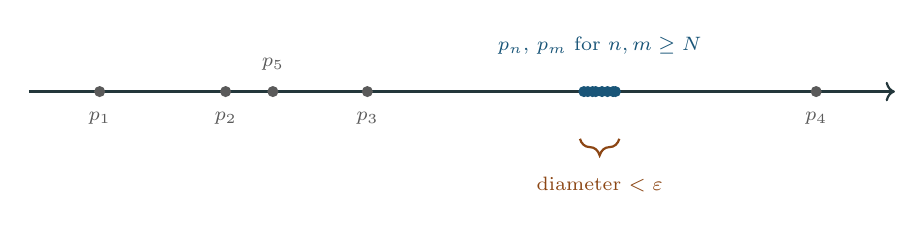
\begin{tikzpicture}[scale=1.0]
    % Number line
    \draw[->, thick, mDarkTeal] (-5.5, 0) -- (5.5, 0);
    % Early scattered terms
    \fill[remcolor] (-4.6, 0) circle (2pt) node[below=4pt]{\scriptsize $p_1$};
    \fill[remcolor] (-3.0, 0) circle (2pt) node[below=4pt]{\scriptsize $p_2$};
    \fill[remcolor] (-1.2, 0) circle (2pt) node[below=4pt]{\scriptsize $p_3$};
    \fill[remcolor] (4.5, 0) circle (2pt) node[below=4pt]{\scriptsize $p_4$};
    \fill[remcolor] (-2.4, 0) circle (2pt) node[above=4pt]{\scriptsize $p_5$};
    % Tail: clustered terms
    \fill[defcolor] (1.6, 0) circle (2pt);
    \fill[defcolor] (1.85, 0) circle (2pt);
    \fill[defcolor] (1.7, 0) circle (2pt);
    \fill[defcolor] (1.95, 0) circle (2pt);
    \fill[defcolor] (1.55, 0) circle (2pt);
    \fill[defcolor] (1.78, 0) circle (2pt);
    \fill[defcolor] (1.92, 0) circle (2pt);
    \fill[defcolor] (1.66, 0) circle (2pt);
    % Bracket showing diameter
    \draw[thick, mAccent, decorate, decoration={brace, amplitude=6pt, mirror}]
      (1.5, -0.6) -- (2.0, -0.6) node[midway, below=10pt]{\scriptsize diameter $< \varepsilon$};
    \node[defcolor, above=10pt] at (1.75, 0) {\scriptsize $p_n,\, p_m$ for $n,m \geq N$};
  \end{tikzpicture}
  \end{center}

  \vspace{0.3em}
  \begin{center}
    \hl{\emph{Past index $N$, all terms fit inside an $\varepsilon$-window.}}
  \end{center}

  \note{
    Here is the visual idea. The arrow is the real line, and the dots
    are the terms of a Cauchy sequence. The early terms, drawn in gray
    and labeled "p" sub 1, "p" sub 2, "p" sub 3, "p" sub 4, "p" sub 5,
    are scattered far apart. As we go further along, the blue dots
    start to cluster: from some index "N" onward, every term lies
    inside a tiny window, and the brace below the window indicates that
    its width is less than epsilon. The Cauchy condition asks that we
    can do this for any epsilon we like, by choosing "N" large enough.
    Notice once again that no target point is marked anywhere on the
    line. The dots are simply huddling together.
  }
\end{frame}

% --- Definition 3.9 ---
\begin{frame}{Definition 3.9: Diameter}
  \begin{defblock}{Definition 3.9 --- Diameter}
    Let $E$ be a nonempty subset of a metric space $X$, and let
    \[
      S = \{\, d(p, q) : p \in E,\; q \in E \,\}.
    \]
    The \alert{diameter} of $E$ is
    \[
      \operatorname{diam} E = \sup S.
    \]
  \end{defblock}

  \vspace{0.4em}
  \hl{\textbf{Intuition:} $\operatorname{diam} E$ is the \emph{largest distance} between two points of $E$.}

  \note{
    To restate the Cauchy condition geometrically we introduce the
    diameter of a set. Look at the set "S" of all distances between
    pairs of points of "E", and take its supremum. That number is
    the diameter, a single value capturing how spread out "E" is.
    Two subtleties are worth flagging. First, we use supremum, not
    maximum, because the largest distance might never be attained.
    Think of an open interval, where points get arbitrarily close
    to the endpoints but never reach them; the diameter is the
    length of the interval, even though no two points realise it.
    Second, if "E" is unbounded, the set of distances has no upper
    bound and the diameter is plus infinity. With this concept in
    hand, the Cauchy condition will become a statement about how
    spread out the tails of the sequence are.
  }
\end{frame}

% --- Cauchy in terms of diameter ---
\begin{frame}{Cauchy in Terms of Diameter}
  \hl{Let $E_N = \{p_N, p_{N+1}, p_{N+2}, \ldots\}$ be the \emph{tail} starting at index $N$.}

  \vspace{0.6em}
  \begin{remblock}{Equivalent Form of the Cauchy Condition}
    \[
      \{p_n\} \text{ is Cauchy} \quad \iff \quad \lim_{N \to \infty} \operatorname{diam} E_N = 0.
    \]
  \end{remblock}

  \vspace{0.6em}
  \hl{\textbf{Why:} $\operatorname{diam} E_N < \varepsilon$ says that any two terms past index $N$ are within $\varepsilon$.}

  \note{
    Combining the last two definitions gives a clean reformulation.
    For each "N", form the tail "E" sub "N" by collecting "p" sub
    "N" and everything that comes after. The sequence is Cauchy
    precisely when the diameters of these tails shrink to zero.
    This is the same Cauchy condition recast: the tail has diameter
    less than epsilon if and only if any two of its members are
    within epsilon of each other. The reformulation is more than
    cosmetic. In the proofs that follow we want to treat tails as
    geometric objects, and diameter is the right measurement of how
    concentrated they have become. The Cauchy condition is, in
    effect, a shrinking-tails condition.
  }
\end{frame}

}

{
\usebackgroundtemplate{%
  
\includegraphics[width=\paperwidth,height=\paperheight,keepaspectratio=false]{chapter_03_bg_03.png}%
}
% =============================================================================
% THEOREM 3.10
% =============================================================================
\section{Diameters and Nested Compacts}

% --- Theorem 3.10: Build 1/2 ---
\begin{frame}{Theorem 3.10: Two Geometric Facts}
  \begin{thmblock}{Theorem 3.10 (a)}
    If $\bar{E}$ is the closure of a set $E$ in a metric space $X$, then
    \[
      \operatorname{diam} \bar{E} = \operatorname{diam} E.
    \]
  \end{thmblock}

  \note{
    Theorem 3.10 records two geometric facts we will need for the
    Cauchy criterion. Part "a" is the simpler one: the closure of
    a set has the same diameter as the set itself. Why should you
    expect this? Closing up adds in the limit points, and every
    newly added point sits arbitrarily close to a point that was
    already in "E". So any pair of points in the closure can be
    approximated by a pair already in "E", with their distance
    approximated too. Approximated, not increased, so the supremum
    of distances cannot grow. The precise argument follows in a
    moment.
  }
\end{frame}

% --- Theorem 3.10: Build 2/2 ---
\begin{frame}{Theorem 3.10: Two Geometric Facts}
  \begin{thmblock}{Theorem 3.10 (a)}
    If $\bar{E}$ is the closure of a set $E$ in a metric space $X$, then
    \[
      \operatorname{diam} \bar{E} = \operatorname{diam} E.
    \]
  \end{thmblock}

  \begin{thmblock}{Theorem 3.10 (b)}
    Let $\{K_n\}$ be a sequence of \alert{nonempty compact} sets in $X$ with
    \[
      K_1 \supset K_2 \supset K_3 \supset \cdots
      \quad\text{and}\quad
      \lim_{n\to\infty} \operatorname{diam} K_n = 0.
    \]
    Then $\bigcap_{n=1}^{\infty} K_n$ consists of \alert{exactly one point}.
  \end{thmblock}

  \note{
    Part "b" is the geometric heart of the section. It says: take a
    nested decreasing sequence of nonempty compact sets whose
    diameters shrink to zero. Then their intersection is a single
    point. Two hypotheses each play a role. Nonemptiness, together
    with compactness, guarantees that the intersection is nonempty,
    by Theorem 2.36 from Chapter 2; without nonemptiness the
    intersection could already be empty after the very first set.
    The diameters shrinking to zero forces the intersection to
    contain at most one point. Together, exactly one point. This is
    the engine that will drive the proof of the Cauchy criterion in
    compact spaces.
  }
\end{frame}

% --- Picture: nested compacts ---
\begin{frame}{Picture: Nested Compacts Pinch to a Point}
  \begin{center}
  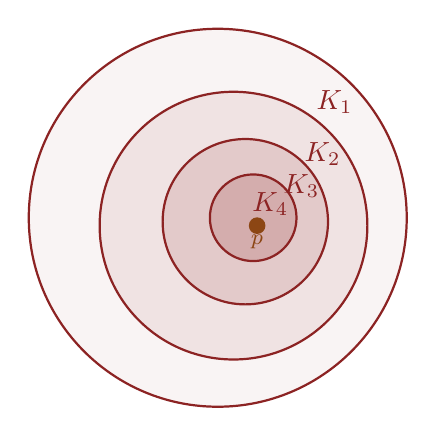
\begin{tikzpicture}[scale=1.0]
    \fill[thmcolor!10, opacity=0.5] (0,0) circle (2.4);
    \draw[thick, thmcolor] (0,0) circle (2.4) node[above right=34pt and 32pt, thmcolor]{$K_1$};
    \fill[thmcolor!20, opacity=0.5] (0.2,-0.1) circle (1.7);
    \draw[thick, thmcolor] (0.2,-0.1) circle (1.7) node[above right=18pt and 22pt, thmcolor]{$K_2$};
    \fill[thmcolor!35, opacity=0.5] (0.35,-0.05) circle (1.05);
    \draw[thick, thmcolor] (0.35,-0.05) circle (1.05) node[above right=5pt and 10pt, thmcolor]{$K_3$};
    \fill[thmcolor!50, opacity=0.5] (0.45,0) circle (0.55);
    \draw[thick, thmcolor] (0.45,0) circle (0.55) node[above right=-3pt and -4pt, thmcolor]{$K_4$};
    \fill[mAccent] (0.5,-0.1) circle (3pt);
    \node[mAccent, below=4pt] at (0.5,0.05) {\footnotesize $p$};
  \end{tikzpicture}
  \begin{hlbox}
    \begin{center}
    \emph{Each $K_n$ is nonempty and compact; $K_{n+1} \subset K_n$; diameters shrink to $0$;\\
    the intersection is a single point.}
    \end{center}
  \end{hlbox}
  \end{center}

  \note{
    Here is the picture behind part "b". The nested sets are drawn
    as decreasing red disks, labeled "K" sub 1 on the outside down
    to "K" sub 4 on the inside, with the shading getting darker as
    we go in. Each set is nonempty, compact, and contained in the
    one before. The diameters are also shrinking; in the limit they
    go to zero. The orange dot in the middle is the unique point
    lying in every set, and that is the only point of the
    intersection. The picture is the only possible behaviour: a
    single point is squeezed out at the end.
  }
\end{frame}

% --- Proof of 3.10(a): Build 1/2 (easy direction) ---
\begin{frame}{Proof of 3.10 (a): $\operatorname{diam} \bar{E} = \operatorname{diam} E$}
  \begin{proofblock}{Easy direction: $\operatorname{diam} E \leq \operatorname{diam} \bar{E}$}
    $E \subset \bar{E}$, so every distance realised in $E$ is realised in $\bar{E}$:
    \[
      \operatorname{diam} E \leq \operatorname{diam} \bar{E}.
    \]
  \end{proofblock}

  \note{
    The proof has two halves. The easy direction is just monotonicity
    of the supremum: "E" is contained in its closure, so every
    distance between two points of "E" is also a distance between two
    points of the closure. Taking suprema, the diameter of "E" is at
    most the diameter of the closure.
  }
\end{frame}

% --- Proof of 3.10(a): Build 2/2 (other direction) ---
\begin{frame}{Proof of 3.10 (a): $\operatorname{diam} \bar{E} = \operatorname{diam} E$}
  \begin{proofblock}{Easy direction: $\operatorname{diam} E \leq \operatorname{diam} \bar{E}$}
    $E \subset \bar{E}$, so $\operatorname{diam} E \leq \operatorname{diam} \bar{E}$.
  \end{proofblock}

  \vspace{0.4em}
  \begin{proofblock}{Other direction: $\operatorname{diam} \bar{E} \leq \operatorname{diam} E$}
    Fix $\varepsilon > 0$, $p, q \in \bar{E}$. Pick $p', q' \in E$ with $d(p,p') < \varepsilon$ and $d(q,q') < \varepsilon$. Then
    \[
      d(p, q) \leq d(p, p') + d(p', q') + d(q', q) < 2\varepsilon + \operatorname{diam} E.
    \]
    Hence $\operatorname{diam} \bar{E} \leq 2\varepsilon + \operatorname{diam} E$ for all $\varepsilon > 0$. \quad $\Box$
  \end{proofblock}

  \note{
    The other direction is the substantive half. Pick any two points
    "p" and "q" of the closure. By the definition of closure, each is
    approximated within epsilon by a point of "E", call them "p"
    prime and "q" prime. The triangle inequality, displayed on the
    slide, routes the distance from "p" to "q" through "p" prime and
    "q" prime, paying twice epsilon of slack and otherwise charging
    only a distance inside "E". Since epsilon was arbitrary, the
    diameter of the closure is at most the diameter of "E", and we
    have equality.
  }
\end{frame}

% --- Proof of 3.10(b): Build 1/2 (intersection is nonempty) ---
\begin{frame}{Proof of 3.10 (b): Intersection Is a Single Point}
  \begin{proofblock}{Step 1 --- intersection is nonempty}
    Each $K_n$ is \alert{nonempty} and \alert{compact}, and $K_n \supset K_{n+1}$, so every finite subfamily has nonempty intersection. By \alert{Theorem 2.36},
    $K = \bigcap_{n=1}^{\infty} K_n \neq \emptyset$.
  \end{proofblock}

  \note{
    The proof splits into two steps. Step 1 produces at least one
    point of the intersection. Here is where both hypotheses on the
    "K" sub "n" pull their weight: each "K" sub "n" is nonempty and
    compact, and they are nested. Any finite subfamily intersects
    in its smallest member, which is nonempty by hypothesis. So the
    family has the finite intersection property, and Theorem 2.36
    from Chapter 2 then gives that the full infinite intersection
    "K" is nonempty.
  }
\end{frame}

% --- Proof of 3.10(b): Build 2/2 (it cannot contain two points) ---
\begin{frame}{Proof of 3.10 (b): Intersection Is a Single Point}
  \begin{proofblock}{Step 1 --- intersection is nonempty}
    Each $K_n$ is \alert{nonempty} and \alert{compact}, and $K_n \supset K_{n+1}$, so every finite subfamily has nonempty intersection. By \alert{Theorem 2.36},
    $K = \bigcap_{n=1}^{\infty} K_n \neq \emptyset$.
  \end{proofblock}

  \vspace{0.4em}
  \begin{proofblock}{Step 2 --- it cannot contain two points}
    If $K$ had two points, $\operatorname{diam} K > 0$. But $K \subset K_n$ for every $n$, so
    \[
      \operatorname{diam} K_n \geq \operatorname{diam} K > 0 \quad \text{for all } n,
    \]
    contradicting $\operatorname{diam} K_n \to 0$. So $K$ is exactly one point. \quad $\Box$
  \end{proofblock}

  \note{
    Step 2 rules out two or more points. Suppose for contradiction
    that "K" had two distinct points. Then the diameter of "K"
    would be strictly positive. But "K" sits inside every "K" sub
    "n", so the diameter of "K" sub "n" is at least the diameter
    of "K" for every "n". That contradicts the assumption that the
    diameters of "K" sub "n" tend to zero. So "K" has exactly one
    point.
  }
\end{frame}

}

{
\usebackgroundtemplate{%
  
\includegraphics[width=\paperwidth,height=\paperheight,keepaspectratio=false]{chapter_03_bg_04.png}%
}
% =============================================================================
% THEOREM 3.11: THE CAUCHY CRITERION
% =============================================================================
\section{The Cauchy Criterion}

% --- Theorem 3.11: Build 1/3 ---
\begin{frame}{Theorem 3.11: Cauchy and Convergent}
  \begin{thmblock}{Theorem 3.11 (a)}
    In any metric space $X$, every \alert{convergent sequence is Cauchy}.
  \end{thmblock}

  \note{
    Theorem 3.11 has three parts. Part "a" is the easy direction
    and holds in any metric space, with no extra assumptions. Every
    convergent sequence is automatically Cauchy. The reason is
    intuitive: if the late terms are crowding inside an
    epsilon-ball around the limit "p", any two of them are within
    twice epsilon of each other by the triangle inequality. So
    crowding around a single point automatically forces crowding
    around each other. Convergence implies Cauchy, with no special
    structure on the space at all.
  }
\end{frame}

% --- Theorem 3.11: Build 2/3 ---
\begin{frame}{Theorem 3.11: Cauchy and Convergent}
  \begin{thmblock}{Theorem 3.11 (a)}
    In any metric space $X$, every \alert{convergent sequence is Cauchy}.
  \end{thmblock}

  \begin{thmblock}{Theorem 3.11 (b)}
    In a \alert{compact} metric space $X$, every Cauchy sequence \alert{converges in $X$}.
  \end{thmblock}

  \note{
    Part "b" is the deep direction, the converse of part "a". It
    needs an extra hypothesis: the ambient metric space "X" must
    be compact. Under that hypothesis, every Cauchy sequence
    converges to a point of "X". The compactness assumption is
    essential. We will soon see that in the rationals, the decimal
    truncations of the square root of 2 form a Cauchy sequence
    that has nowhere to converge, because the would-be limit is
    irrational and lies outside the space. Compactness is the
    structural assumption that closes off this kind of escape.
  }
\end{frame}

% --- Theorem 3.11: Build 3/3 ---
\begin{frame}{Theorem 3.11: Cauchy and Convergent}
  \begin{thmblock}{Theorem 3.11 (a)}
    In any metric space $X$, every \alert{convergent sequence is Cauchy}.
  \end{thmblock}

  \begin{thmblock}{Theorem 3.11 (b)}
    In a \alert{compact} metric space $X$, every Cauchy sequence \alert{converges in $X$}.
  \end{thmblock}

  \begin{thmblock}{Theorem 3.11 (c)}
    In $\mathbb{R}^k$, every Cauchy sequence \alert{converges}.
  \end{thmblock}

  \note{
    Part "c" specialises to euclidean space "R" to the "k". Every
    Cauchy sequence in "R" to the "k" converges, no compactness
    assumption needed on the ambient space. This is the Cauchy
    criterion in its most familiar form. The proof of part "c" is a
    quick reduction to part "b": a Cauchy sequence is bounded, and
    bounded subsets of "R" to the "k" sit inside compact sets, so
    part "b" applies. We will write this all out below.
  }
\end{frame}

% --- Cauchy criterion remark ---
\begin{frame}{Why This Theorem Is Powerful}
  \begin{remblock}{The Cauchy Criterion}
    The convergence definition involves the limit. \\
    The Cauchy condition does not.
    \medskip
    \begin{itemize}
      \item In $\mathbb{R}^k$: \;\; $\{p_n\}$ converges \;\; $\iff$ \;\; $\{p_n\}$ is Cauchy.
      \item Decide convergence \alert{without} producing the limit.
    \end{itemize}
  \end{remblock}

  \note{
    Pause to take in the punch line. Convergence as we defined it
    refers to a limit, but the Cauchy condition refers only to the
    sequence. In "R" to the "k" the two are equivalent, so we can
    decide convergence without ever producing the limit. This pair
    of equivalent statements has its own name: the Cauchy criterion
    for convergence. With the criterion stated, we now turn to the
    proof.
  }
\end{frame}

% --- Proof 3.11 (a) ---
\begin{frame}{Proof of 3.11 (a): Convergent $\Rightarrow$ Cauchy}
  \begin{proofblock}{Triangle Inequality}
    Suppose $p_n \to p$. Given $\varepsilon > 0$, choose $N$ with $d(p_n, p) < \varepsilon$ for $n \geq N$. Then for $n, m \geq N$,
    \[
      d(p_n, p_m) \leq d(p_n, p) + d(p, p_m) < 2\varepsilon. \quad \Box
    \]
  \end{proofblock}

  \vspace{0.4em}
  \hl{\textbf{Idea:} Triangle inequality routes any two terms through the limit.}

  \note{
    The proof of part "a" is a one-line application of the
    triangle inequality. Pick "N" so that every term past index
    "N" is within epsilon of the limit "p". The displayed
    inequality then routes any two such terms through "p", paying
    epsilon on each leg, for less than twice epsilon total. The
    arbitrary epsilon and the resulting twice epsilon both shrink
    to zero, so the Cauchy condition holds. Notice we have not
    used anything special about the ambient space; this argument
    works in every metric space, which is exactly why part "a"
    holds without any extra hypothesis.
  }
\end{frame}

% --- Proof 3.11 (b) Strategy ---
\begin{frame}{Proof Strategy: 3.11 (b)}
  \begin{hlbox}
    \textbf{Setting:} $X$ compact, $\{p_n\}$ Cauchy. Want: $p_n \to p$ for some $p \in X$.

    \vspace{0.5em}
    \textbf{Plan:}
    \begin{enumerate}
      \item Form tails $E_N = \{p_N, p_{N+1}, \ldots\}$ and their closures $\bar{E}_N$.
      \item Show $\operatorname{diam} \bar{E}_N \to 0$ (use Theorem 3.10 (a) + Cauchy condition).
      \item Each $\bar{E}_N$ is compact and $\bar{E}_N \supset \bar{E}_{N+1}$ (nested compacts).
      \item Apply Theorem 3.10 (b): a unique $p \in \bigcap_N \bar{E}_N$.
      \item Show $p_n \to p$.
    \end{enumerate}
  \end{hlbox}

  \note{
    The proof of part "b" deserves a roadmap. The challenge is to
    produce a limit "p" without ever being told what "p" is. The
    strategy is to corner "p" geometrically. The closure of each
    tail forms a region the sequence can never escape; compactness
    makes those regions compact, and the Cauchy condition makes
    them shrink. Theorem 3.10 part "b" then squeezes out a single
    point common to every region, and that point must be the
    limit. The five bullets on the slide implement this plan
    using only tools we already developed in Chapter 2 and earlier
    in this section.
  }
\end{frame}

% --- Proof 3.11 (b) Step 1: tails and diameters ---
\begin{frame}{Proof of 3.11 (b) --- Step 1: Tails and Diameters}
  \hl{Define $E_N = \{p_N, p_{N+1}, p_{N+2}, \ldots\}$ for each $N$.}

  \vspace{0.5em}
  \begin{proofblock}{Cauchy $\Longrightarrow$ shrinking diameters}
    \[
      \{p_n\} \text{ Cauchy}
      \;\Longrightarrow\;
      \operatorname{diam} E_N \to 0
      \;\stackrel{\text{Thm 3.10 (a)}}{\Longrightarrow}\;
      \operatorname{diam} \bar{E}_N \to 0. \tag{3}
    \]
  \end{proofblock}

  \note{
    Step 1 turns the Cauchy condition into a geometric statement.
    For each "N", the tail "E" sub "N" collects every term from
    index "N" onward. We saw a few slides ago that being Cauchy
    means the diameters of these tails shrink to zero. We now want
    closures, not the tails themselves, because closures are
    closed and we will need closedness in the next step. Theorem
    3.10 part "a" tells us that closure does not change diameter,
    so the closures shrink to zero too. The conclusion, marked as
    equation 3 on the slide, is the geometric form of the Cauchy
    hypothesis we will use through the rest of the proof.
  }
\end{frame}

% --- Proof 3.11 (b) Step 2: nested compacts ---
\begin{frame}{Proof of 3.11 (b) --- Step 2: Nested Compacts}
  \begin{proofblock}{Closures are nonempty, compact, nested}
    Each $\bar{E}_N$ contains $p_N$, hence is \alert{nonempty}.
    \medskip

    $\bar{E}_N$ is closed in compact $X$, hence \alert{compact} (Theorem 2.35).
    \medskip

    $E_N \supset E_{N+1}$ gives $\bar{E}_N \supset \bar{E}_{N+1}$.
  \end{proofblock}

  \vspace{0.4em}
  \begin{proofblock}{A unique limit candidate}
    All hypotheses of Theorem 3.10 (b) hold, so there is a \alert{unique $p \in X$} with
    \[
      p \in \bar{E}_N \quad \text{for every } N.
    \]
  \end{proofblock}

  \note{
    Step 2: line up the hypotheses for Theorem 3.10 part "b". Each
    closure "E" sub "N" bar contains the term "p" sub "N", so it
    is nonempty. It is closed in the compact space "X", so by
    Theorem 2.35 from Chapter 2 it is also compact. The closures
    are nested, because the tails themselves are. Combined with
    equation 3 from Step 1, which gave the diameters tending to
    zero, every hypothesis of Theorem 3.10 part "b" is satisfied,
    and we conclude there is a unique point "p" lying in every
    closure. This "p" is our candidate limit.
  }
\end{frame}

% --- Proof 3.11 (b) Step 3: convergence ---
\begin{frame}{Proof of 3.11 (b) --- Step 3: $p_n \to p$}
  \begin{proofblock}{Closing the argument}
    Let $\varepsilon > 0$. By (3), choose $N_0$ with $\operatorname{diam} \bar{E}_N < \varepsilon$ for $N \geq N_0$.

    \vspace{0.3em}
    Since $p \in \bar{E}_N$, every $q \in \bar{E}_N$ satisfies $d(p, q) < \varepsilon$.

    \vspace{0.3em}
    In particular, for $n \geq N_0$,
    \[
      d(p, p_n) < \varepsilon, \quad \text{i.e.,} \quad p_n \to p. \quad \Box
    \]
  \end{proofblock}

  \note{
    Step 3 closes the loop and shows that "p" really is the limit.
    Fix any positive epsilon. Equation 3 from Step 1 lets us pick
    a cutoff "N" sub 0 past which the tail closures all have
    diameter less than epsilon. Here is the punch line: "p" sits
    inside that tiny closure, and so does every term "p" sub "n"
    for "n" past the cutoff. Two points sharing a set of diameter
    less than epsilon must be within epsilon of each other, so "p"
    sub "n" is within epsilon of "p". That is convergence, and
    part "b" is done. The whole argument was an application of the
    nested-compacts squeezing principle from Theorem 3.10.
  }
\end{frame}

% --- Proof 3.11 (c) ---
\begin{frame}{Proof of 3.11 (c): Cauchy in $\mathbb{R}^k$ Converges}
  \begin{proofblock}{Reduce to part (b)}
    Let $\{\mathbf{x}_n\}$ be Cauchy in $\mathbb{R}^k$. Some tail $E_N$ has $\operatorname{diam} E_N < 1$, so the range
    \[
      \{\mathbf{x}_n : n \geq 1\} = E_N \cup \{\mathbf{x}_1, \ldots, \mathbf{x}_{N-1}\}
    \]
    is \alert{bounded}. By Theorem 2.41, its closure is \alert{compact}.

    \vspace{0.3em}
    Apply (b) inside this compact set. \quad $\Box$
  \end{proofblock}

  \note{
    Part "c" is now a quick consequence of part "b". Take a Cauchy
    sequence in "R" to the "k". Because it is Cauchy, some tail has
    diameter less than 1, and the whole range of the sequence is the
    union of that bounded tail with finitely many earlier terms,
    which is itself bounded. By Theorem 2.41 from Chapter 2, every
    bounded subset of "R" to the "k" has compact closure. So the
    sequence lives inside a compact subset of "R" to the "k". Part
    "b" applies inside that compact set and gives convergence.
  }
\end{frame}

}

{
\usebackgroundtemplate{%
  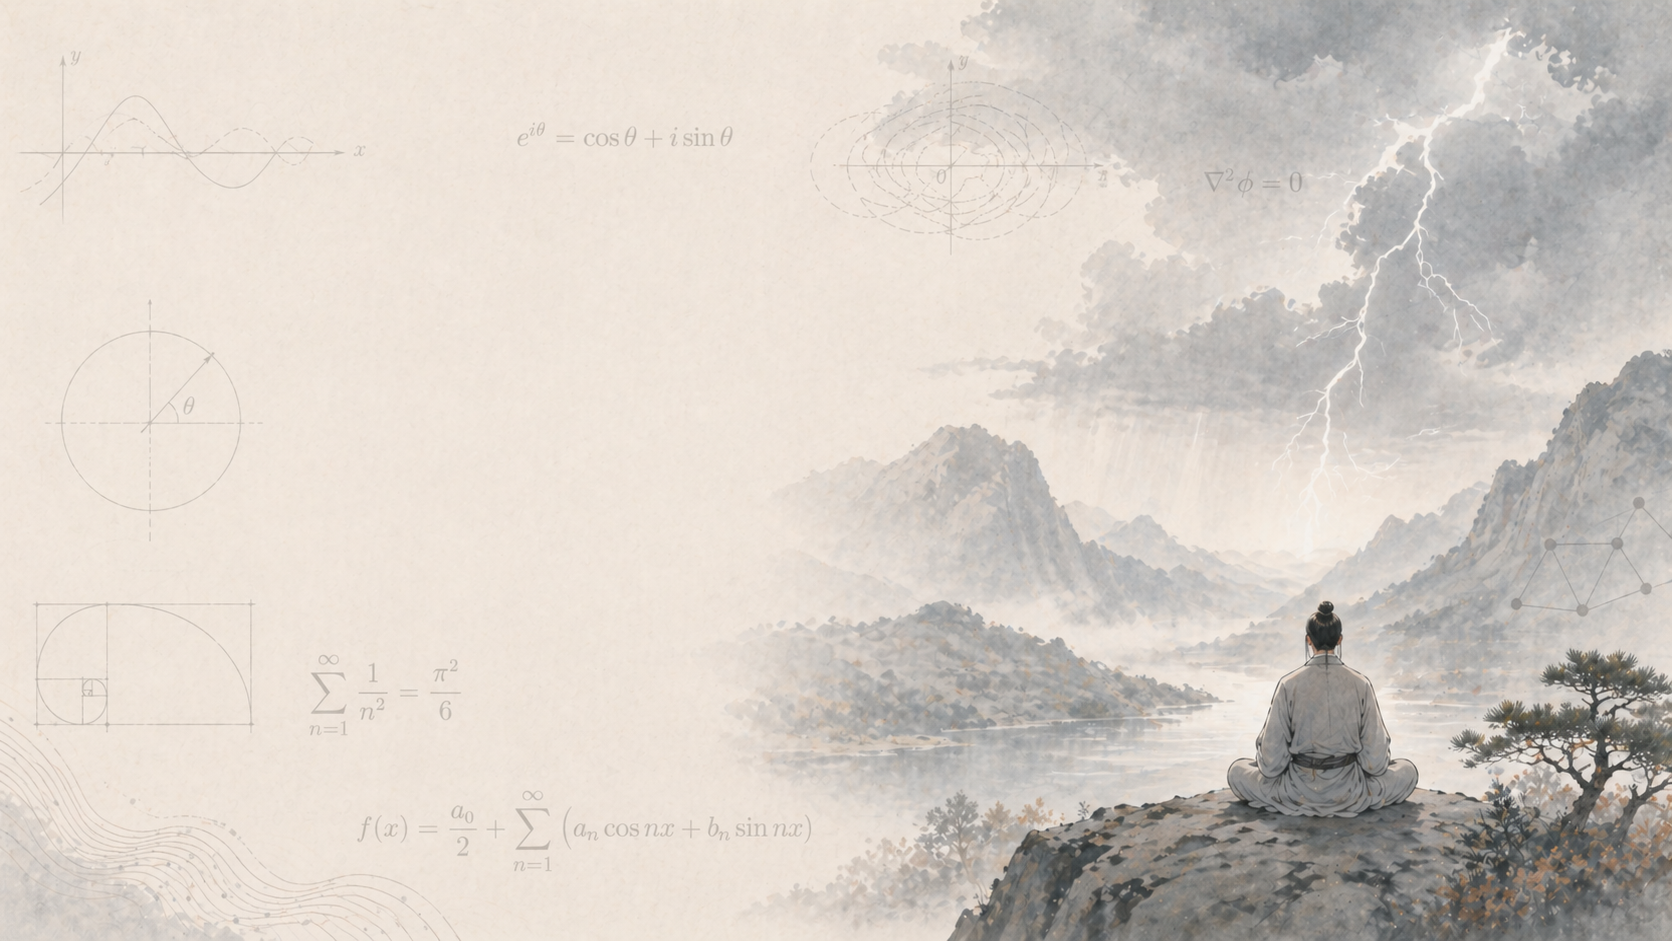
\includegraphics[width=\paperwidth,height=\paperheight,keepaspectratio=false]{chapter_03_bg_05.png}%
}
% =============================================================================
% COMPLETENESS
% =============================================================================
\section{Complete Metric Spaces}

% --- Definition 3.12 ---
\begin{frame}{Definition 3.12: Complete Metric Space}
  \begin{defblock}{Definition 3.12 --- Complete}
    A metric space in which \alert{every Cauchy sequence converges} is \alert{complete}.
  \end{defblock}

  \vspace{0.5em}
  \begin{hlbox}
    Theorem 3.11 reads:
    \begin{itemize}
      \item Every \alert{compact metric space} is complete.
      \item Every \alert{Euclidean space} $\mathbb{R}^k$ is complete.
    \end{itemize}
  \end{hlbox}

  \note{
    With Theorem 3.11 in hand we can name the property. A metric
    space is complete if every Cauchy sequence in it converges to a
    point of the space. Theorem 3.11 then reads cleanly: every
    compact metric space is complete, and every euclidean space is
    complete. The word complete is well chosen. A Cauchy sequence
    is a sequence that is trying to converge somewhere. If the
    would-be limit is missing from the space, the space has a hole
    that the sequence falls through. Completeness says there are no
    such holes; every limit a sequence wants is actually present.
    The deeper reason the real line is the right setting for
    analysis comes down to this single property.
  }
\end{frame}

% --- Closed in complete is complete ---
\begin{frame}{Closed Subsets of a Complete Space Are Complete}
  \begin{thmblock}{Inheritance}
    Every \alert{closed subset $E$} of a complete metric space $X$ is itself complete.
  \end{thmblock}

  \vspace{0.5em}
  \begin{hlbox}
    \textbf{Why:}
    \begin{itemize}
      \item A Cauchy sequence in $E$ is Cauchy in $X$, so it converges to $p \in X$.
      \item $E$ is closed $\Rightarrow$ $p \in E$.
    \end{itemize}
  \end{hlbox}

  \note{
    Theorem 3.11 also has an important corollary: every closed
    subset of a complete metric space is itself complete. The
    argument is short. A Cauchy sequence in "E" is in particular
    Cauchy in the larger space "X", which is complete, so the
    sequence converges to some point "p" in "X". Now "E" is closed,
    so it contains all its limit points, and "p" must lie in "E".
    Thus every Cauchy sequence in "E" converges in "E", which is
    the completeness of "E".
  }
\end{frame}

% --- Example: Q is not complete ---
\begin{frame}{Example: $\mathbb{Q}$ Is Not Complete}
  \begin{exblock}{A Cauchy sequence in $\mathbb{Q}$ with no rational limit}
    Let $r_n$ be the truncation of $\sqrt{2}$ to $n$ decimal places:
    \[
      r_1 = 1.4,\; r_2 = 1.41,\; r_3 = 1.414,\; r_4 = 1.4142,\; \ldots
    \]
    \begin{itemize}
      \item Each $r_n \in \mathbb{Q}$ and $|r_n - r_m| \leq 10^{-\min(n,m)} \to 0$ \;\;($\{r_n\}$ is \alert{Cauchy}).
      \item In $\mathbb{R}$, $r_n \to \sqrt{2}$. But $\sqrt{2} \notin \mathbb{Q}$.
    \end{itemize}
    So $\{r_n\}$ is Cauchy in $\mathbb{Q}$ \alert{with no limit in $\mathbb{Q}$}.
  \end{exblock}

  \note{
    Here is a textbook example of a metric space that is not
    complete. Take the rational numbers with the usual distance,
    absolute value of the difference. The decimal truncations of
    the square root of 2, namely 1.4, 1.41, 1.414, 1.4142, and so
    on, are all rational, and they form a Cauchy sequence because
    any two of them agree up to a power of one tenth. But in the
    real line they converge to the square root of 2, which is not
    rational. So this Cauchy sequence in the rationals has no limit
    inside the rationals. The rationals fail to be complete; the
    real line was specifically constructed to fix this.
  }
\end{frame}

}

{
\usebackgroundtemplate{%
  
\includegraphics[width=\paperwidth,height=\paperheight,keepaspectratio=false]{chapter_03_bg_06.png}%
}
% =============================================================================
% MONOTONIC SEQUENCES
% =============================================================================
\section{Monotonic Sequences in $\mathbb{R}$}

% --- Setup remark before Definition 3.13 ---
\begin{frame}{One Important Case: Monotonic Sequences}
  \begin{remblock}{Bounded vs. Convergent}
    \begin{itemize}
      \item Every convergent sequence in $\mathbb{R}^k$ is bounded \;\;(Theorem 3.2 (c)).
      \item Bounded sequences in $\mathbb{R}^k$ \alert{need not} converge \;\;(e.g., $(-1)^n$).
      \item \alert{Special case:} for monotonic sequences in $\mathbb{R}$, bounded $\iff$ convergent.
    \end{itemize}
  \end{remblock}

  \note{
    Before the next definition, contrast convergence with
    boundedness. We already know that in "R" to the "k", every
    convergent sequence is bounded; this is Theorem 3.2 part "c"
    from Section 1. The converse fails in general: the alternating
    sequence minus one to the "n" is bounded but does not converge.
    There is, however, one important case in which convergence and
    boundedness coincide, namely monotonic sequences on the real
    line. That is the content of Theorem 3.14, which we are about
    to state.
  }
\end{frame}

% --- Definition 3.13 ---
\begin{frame}{Definition 3.13: Monotonic Sequences}
  \begin{defblock}{Definition 3.13}
    A sequence $\{s_n\}$ of real numbers is
    \begin{itemize}
      \item \alert{monotonically increasing} if $s_n \leq s_{n+1}$ for all $n$;
      \item \alert{monotonically decreasing} if $s_n \geq s_{n+1}$ for all $n$.
    \end{itemize}
    A sequence is \emph{monotonic} if it is increasing or decreasing.
  \end{defblock}

  \note{
    Definition 3.13 just names what we already had in mind: a
    sequence climbs if each term is at most the next, and falls if
    each term is at least the next. The inequalities are non-strict,
    so the sequence is allowed to stay put for a step or two without
    disqualifying itself; constant sequences count as both
    increasing and decreasing. Why isolate this class? Because
    monotonic sequences are well behaved enough that, as we will
    see in Theorem 3.14, the question of convergence reduces to the
    much simpler question of boundedness.
  }
\end{frame}

% --- Theorem 3.14 ---
\begin{frame}{Theorem 3.14: Bounded $\iff$ Convergent for Monotonic}
  \begin{thmblock}{Theorem 3.14}
    Suppose $\{s_n\}$ is monotonic. Then
    \[
      \{s_n\} \text{ converges} \quad \iff \quad \{s_n\} \text{ is bounded}.
    \]
  \end{thmblock}

  \vspace{0.5em}
  \begin{hlbox}
    \textbf{Forward:} Theorem 3.2 (c).

    \vspace{0.3em}
    \textbf{Reverse:} Use the \alert{least upper bound property} of $\mathbb{R}$.
  \end{hlbox}

  \note{
    Here is the theorem itself. If a sequence of real numbers is
    monotonic, then convergence and boundedness are equivalent. The
    forward direction, that a convergent sequence is bounded, is
    Theorem 3.2 part "c" again, and holds with no monotonicity
    assumption. The reverse direction is the content. We will see
    that the supremum of the range of an increasing bounded
    sequence is in fact its limit. The least upper bound property of
    the real line, established in Chapter 1, is exactly the tool we
    need.
  }
\end{frame}

% --- Picture: increasing bounded sequence ---
\begin{frame}{Picture: Increasing and Bounded $\Rightarrow$ Climbs to the sup}
  \begin{center}
  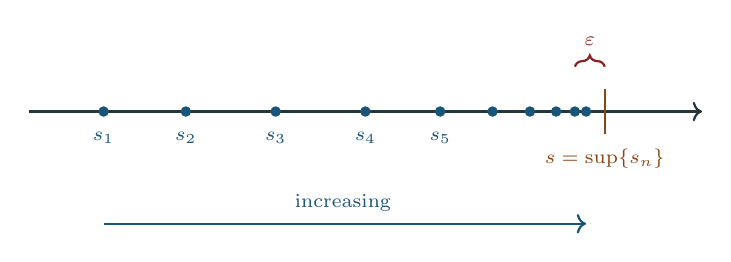
\begin{tikzpicture}[scale=0.95]
    % Number line
    \draw[->, thick, mDarkTeal] (-0.5, 0) -- (8.5, 0);
    % Sequence terms (increasing)
    \fill[defcolor] (0.5, 0) circle (2pt) node[below=4pt]{\scriptsize $s_1$};
    \fill[defcolor] (1.6, 0) circle (2pt) node[below=4pt]{\scriptsize $s_2$};
    \fill[defcolor] (2.8, 0) circle (2pt) node[below=4pt]{\scriptsize $s_3$};
    \fill[defcolor] (4.0, 0) circle (2pt) node[below=4pt]{\scriptsize $s_4$};
    \fill[defcolor] (5.0, 0) circle (2pt) node[below=4pt]{\scriptsize $s_5$};
    \fill[defcolor] (5.7, 0) circle (2pt);
    \fill[defcolor] (6.2, 0) circle (2pt);
    \fill[defcolor] (6.55, 0) circle (2pt);
    \fill[defcolor] (6.8, 0) circle (2pt);
    \fill[defcolor] (6.95, 0) circle (2pt);
    % Supremum
    \draw[thick, mAccent] (7.2, -0.3) -- (7.2, 0.3);
    \node[mAccent, below=2pt] at (7.2, -0.3) {\scriptsize $s = \sup\{s_n\}$};
    % Epsilon window
    \draw[thick, thmcolor, decorate, decoration={brace, amplitude=4pt}]
      (6.8, 0.6) -- (7.2, 0.6) node[midway, above=4pt]{\scriptsize $\varepsilon$};
    % Arrow showing increase
    \draw[->, thick, defcolor] (0.5, -1.5) -- (6.95, -1.5);
    \node[defcolor, below=2pt] at (3.7, -0.9) {\scriptsize increasing};
  \end{tikzpicture}
  \end{center}

  \vspace{0.2em}
  \begin{center}
    \hl{\emph{Past index $N$, $s_n$ enters the strip $(s - \varepsilon, s]$ and never leaves.}}
  \end{center}

  \note{
    Here is the picture behind the proof. The arrow is the real
    line. The blue dots, labeled "s" sub 1, "s" sub 2, "s" sub 3,
    and so on, march steadily to the right because the sequence is
    increasing. The orange tick marks the supremum of the range of
    the sequence, which we are calling "s". The brace at the top
    marks an epsilon window just to the left of "s". Once any term
    enters that window, every subsequent term must also be in the
    window: it cannot fall back, because the sequence is
    increasing, and it cannot exceed "s", because "s" is an upper
    bound. So from some index "N" onward, every term lies between
    "s" minus epsilon and "s", which means the sequence converges
    to "s".
  }
\end{frame}

% --- Proof 3.14: Build 1/2 (setup) ---
\begin{frame}{Proof of Theorem 3.14 (Increasing Case)}
  \begin{proofblock}{Setup}
    Suppose $s_n \leq s_{n+1}$ and $\{s_n\}$ is bounded. \\
    Let $E = \{s_n : n \geq 1\}$ and $s = \sup E$.

    \vspace{0.3em}
    Then $s_n \leq s$ for every $n$.
  \end{proofblock}

  \note{
    We prove the increasing case; the decreasing case is the same
    argument with infimum in place of supremum. Assume the sequence
    is increasing and bounded. Let "E" be the set of terms. Because
    "E" is a nonempty bounded subset of the real line, the least
    upper bound property guarantees a supremum, which we call "s".
    Every term of the sequence is at most "s" by the definition of
    supremum.
  }
\end{frame}

% --- Proof 3.14: Build 2/2 (main argument) ---
\begin{frame}{Proof of Theorem 3.14 (Increasing Case)}
  \begin{proofblock}{Setup}
    $E = \{s_n : n \geq 1\}$, \;\; $s = \sup E$, \;\; $s_n \leq s$ for all $n$.
  \end{proofblock}

  \vspace{0.3em}
  \begin{proofblock}{The supremum is the limit}
    Fix $\varepsilon > 0$. Since $s - \varepsilon < s$, $s - \varepsilon$ is not an upper bound of $E$, so
    \[
      \exists\, N: \;\; s - \varepsilon < s_N \leq s.
    \]
    Since $\{s_n\}$ increases, for every $n \geq N$:
    \[
      s - \varepsilon < s_N \leq s_n \leq s. \quad \Longrightarrow \quad s_n \to s. \quad \Box
    \]
  \end{proofblock}

  \note{
    Now the main argument. Fix any positive epsilon. The number "s"
    minus epsilon is strictly less than "s", so it cannot be an
    upper bound of "E"; some term "s" sub "N" exceeds it. Because
    the sequence is increasing, once we pass index "N" we stay
    above "s" sub "N", and we never climb past the upper bound "s".
    So for every "n" at least "N", the term "s" sub "n" lies in
    the half-open interval from "s" minus epsilon up to "s". That
    is exactly convergence to "s".
  }
\end{frame}

}

{
\usebackgroundtemplate{%
  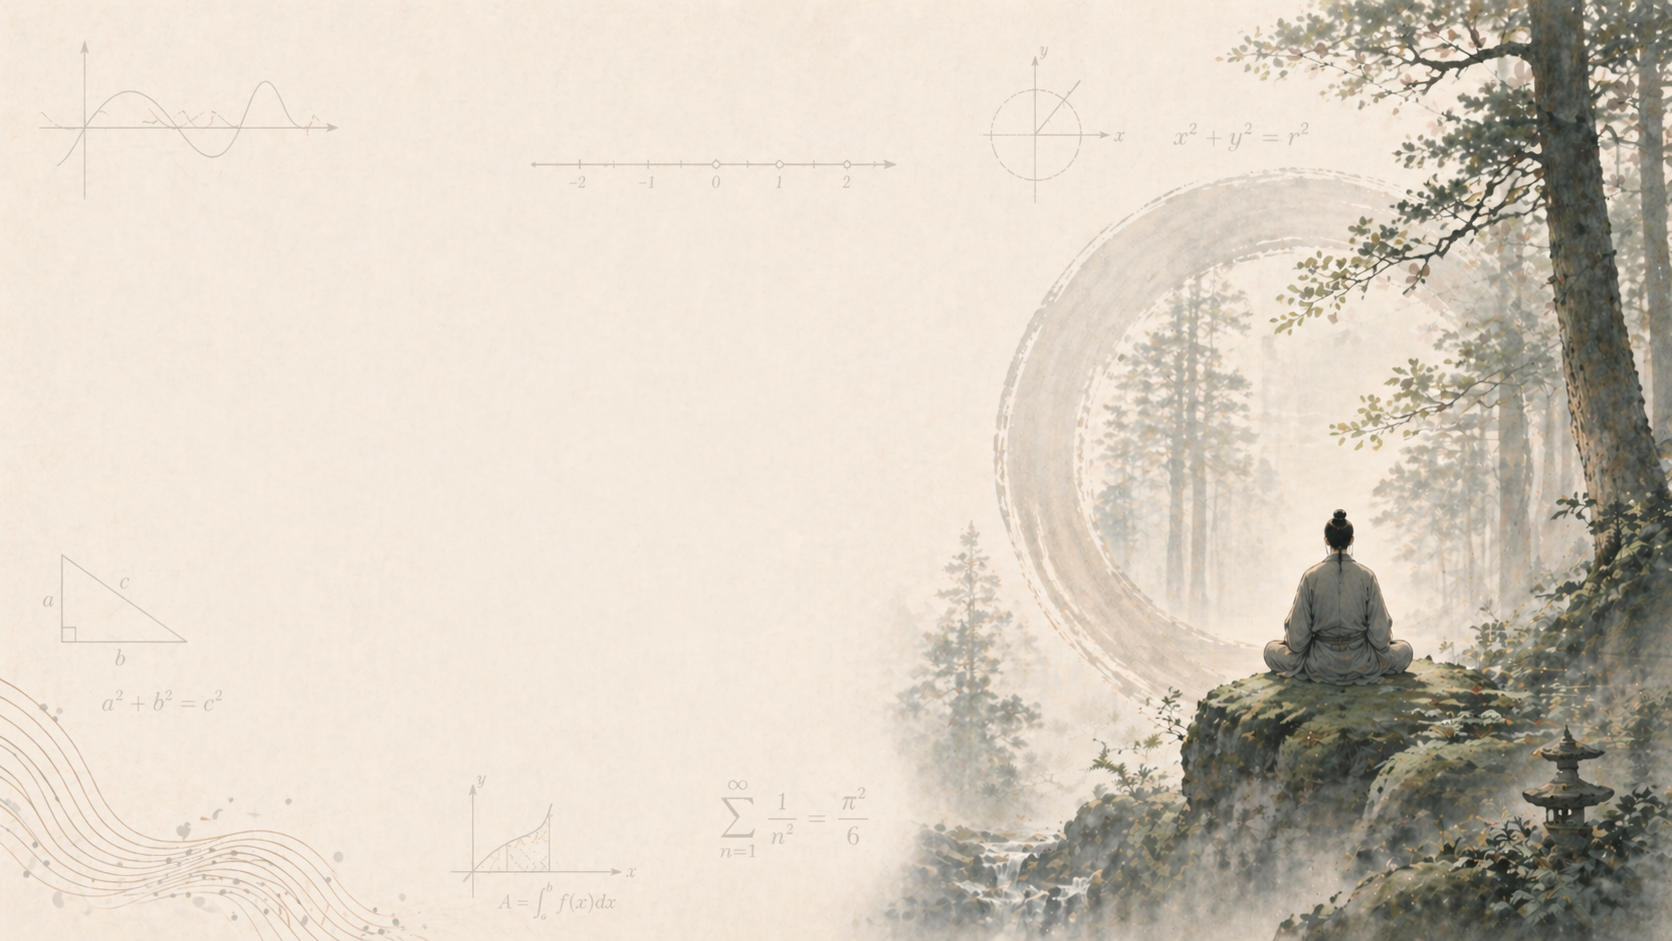
\includegraphics[width=\paperwidth,height=\paperheight,keepaspectratio=false]{chapter_03_bg_07.png}%
}
% =============================================================================
% SUMMARY
% =============================================================================
\section{Summary}

% --- Summary: Build 1/4 ---
\begin{frame}{Summary}
  \begin{hlbox}
    \textbf{Key takeaways from this section:}
    \begin{itemize}
      \item Definition 3.8: $\{p_n\}$ is \alert{Cauchy} if any two late terms are within $\varepsilon$.
    \end{itemize}
  \end{hlbox}

  \note{
    Let us recap. The first key takeaway is the new definition.
    A sequence is Cauchy if, for every positive epsilon, there is a
    cutoff index past which any two terms are within epsilon of
    each other. Crucially, the definition makes no reference to a
    target limit; it only uses distances between terms of the
    sequence.
  }
\end{frame}

% --- Summary: Build 2/4 ---
\begin{frame}{Summary}
  \begin{hlbox}
    \textbf{Key takeaways from this section:}
    \begin{itemize}
      \item Definition 3.8: $\{p_n\}$ is \alert{Cauchy} if any two late terms are within $\varepsilon$.
      \item Theorem 3.11: in compact $X$ (and in $\mathbb{R}^k$), \alert{Cauchy $\iff$ convergent}.
    \end{itemize}
  \end{hlbox}

  \note{
    The second takeaway is Theorem 3.11, the Cauchy criterion. In
    any compact metric space, and in particular in "R" to the "k",
    being Cauchy is equivalent to being convergent. This lets us
    decide convergence without producing a limit, which is one of
    the most useful tricks in analysis.
  }
\end{frame}

% --- Summary: Build 3/4 ---
\begin{frame}{Summary}
  \begin{hlbox}
    \textbf{Key takeaways from this section:}
    \begin{itemize}
      \item Definition 3.8: $\{p_n\}$ is \alert{Cauchy} if any two late terms are within $\varepsilon$.
      \item Theorem 3.11: in compact $X$ (and in $\mathbb{R}^k$), \alert{Cauchy $\iff$ convergent}.
      \item Definition 3.12: a metric space is \alert{complete} if every Cauchy sequence converges.
    \end{itemize}
  \end{hlbox}

  \note{
    The third takeaway is Definition 3.12. A metric space is
    complete if every Cauchy sequence in it converges. Theorem 3.11
    says that compact metric spaces and euclidean spaces are
    complete. The rationals are not complete; they have Cauchy
    sequences that try to converge to irrational numbers.
    Completeness is the absence of holes, and it is the central
    structural property that makes the real line so useful for
    analysis.
  }
\end{frame}

% --- Summary: Build 4/4 ---
\begin{frame}{Summary}
  \begin{hlbox}
    \textbf{Key takeaways from this section:}
    \begin{itemize}
      \item Definition 3.8: $\{p_n\}$ is \alert{Cauchy} if any two late terms are within $\varepsilon$.
      \item Theorem 3.11: in compact $X$ (and in $\mathbb{R}^k$), \alert{Cauchy $\iff$ convergent}.
      \item Definition 3.12: a metric space is \alert{complete} if every Cauchy sequence converges.
      \item Theorem 3.14: monotonic sequences in $\mathbb{R}$ \alert{converge $\iff$ bounded}.
    \end{itemize}

    \vspace{0.5em}
    \textbf{Coming up next:} \emph{Upper and Lower Limits} --- naming the two
    extreme cluster points of any real sequence.
  \end{hlbox}

  \note{
    The fourth takeaway is Theorem 3.14, our small but very useful
    result for monotonic sequences. A monotonic sequence on the
    real line converges if and only if it is bounded, and the limit
    is either the supremum, in the increasing case, or the
    infimum, in the decreasing case. Coming up next is Section 4
    on upper and lower limits, where we extend the idea of a limit
    to two related quantities, the limit superior and the limit
    inferior, which always exist for any real sequence and capture
    the two extreme cluster points. Thank you for following along,
    and see you in the next section.
  }
\end{frame}
}

\end{document}
